%%%%%%%%%%%%%%%%%%%%%%%%
%
% $Autor: Hemanth Jadiswami Prabhakaran $
% $Datum: 2026-09-12 $
% $Pfad: GitHub/MBIDA_Thesis/report/Contents/General/en/06ApplicationDevelopment.tex $
% $Version: 1 $
%
% $Project: MBIDA Thesis $
%
%%%%%%%%%%%%%%%%%%%%%%%%

\chapter{Application Development}
\label{chap:appDevelopment}

This chapter documents how the design decisions set out in Chapter ~\ref{chap:methodology} were built: fitting the three base forecasting models (Section~\ref{sec:modelFitting}), clipping their negative forecasts to zero before reconciliation (Section~\ref{sec:clippingImplementation}), applying the three reconciliation methods (Section~\ref{sec:reconciliationImplementation}), combining the resulting forecast tables and attaching ground truth (Section~\ref{sec:combiningResults}), the pipeline's overall developer-facing flow (Section~\ref{sec:developerDocumentation}), the naming, parameter, and error-handling conventions that run through the code (Section~\ref{sec:namingConventions}), and the pipeline's built-in test protocol (Section~\ref{sec:testingValidation}). The forecasting and reconciliation methods themselves were introduced in Chapter~\ref{chap:domainML}, and why each configuration choice was made is covered in Chapter~\ref{chap:methodology}; this chapter cross-references those decisions rather than re-arguing them. Code organisation and reproducibility concerns that span the whole repository, including \texttt{Code/config.py} itself, are addressed in Chapter~\ref{chap:devToDeployment}, and the accuracy figures produced by this implementation are reported in Chapter~\ref{chap:evaluation}.

\section{Model Fitting}
\label{sec:modelFitting}

All three base models are fitted through a single \texttt{StatsForecast} instance, configured once and reused for both forecast horizons described below:

\begin{Python}
	sf = StatsForecast(
	models=[
	HistoricAverage(alias="histavg"),
	AutoETS(season_length=SEASON_LENGTH, alias="ets"),
	Theta(season_length=SEASON_LENGTH, alias="theta"),
	],
	freq="MS",
	n_jobs=-1,
	fallback_model=HistoricAverage(),
	)
\end{Python}

\texttt{SEASON\_LENGTH} is read from \texttt{config.py} rather than hard-coded here; the rationale for setting it to 12 is given in Section~\ref{sec:seasonLength} and is not repeated here. \texttt{fallback\_model=HistoricAverage()} is a safety net: across more than 30,000 series, some are too short, too sparse, or too irregular for ETS or Theta to fit successfully, and rather than letting the whole run fail on one such series, that series is silently given the HistoricAverage forecast instead. How often this actually happens is measured by the fallback-rate check in Section~\ref{sec:testingValidation}.

Two separate forecasts are produced from this configuration. The test forecast is trained on the training period only and scored against the withheld test-period actuals, over a 12-month horizon (2015-01 to 2016-01). The live forecast is trained on the training and test periods combined and produces a 7-month horizon (2016-01 to 2016-07) with no ground truth to check against, consistent with the live-window definition in Section~\ref{sec:timeWindows}.

\section{Clipping Negative Base Forecasts}
\label{sec:clippingImplementation}

Every base forecast column is clipped at zero, for both the test and live forecast tables, immediately after fitting and before any reconciliation runs:

\begin{Python}
	for _df in (pred_test, pred_live):
	for _col in ["histavg", "ets", "theta"]:
	_n_clipped = (_df[_col] < 0).sum()
	_df[_col] = _df[_col].clip(lower=0)
\end{Python}

The fairness argument for why this step exists -- so that BottomUpSparse and MinTraceSparse start from the same, already-nonnegative base forecasts rather than one implicitly benefiting from a nonnegativity floor the other does not have -- is given in Section~\ref{sec:clippingRationale} and is not repeated here. HistoricAverage, being a simple mean of nonnegative sales figures, never produces a negative value and is consequently never clipped. On the test set, 2,300 ETS values and 16,345 Theta values are clipped; on the live set, the corresponding counts are 712 and 6,752. The larger Theta counts, on both horizons, follow directly from the method's long-term trend line, which is more willing than ETS's exponential smoothing to extrapolate a downward trend through zero on a declining series.

\section{Reconciliation Implementation}
\label{sec:reconciliationImplementation}

A single \texttt{HierarchicalReconciliation} instance applies all three reconciliation methods together:

\begin{Python}
	reconciler = HierarchicalReconciliation(reconcilers=[
	BottomUpSparse(),
	MinTraceSparse(method="wls_struct", nonnegative=True),
	TopDownSparse(method="proportion_averages"),
	])
\end{Python}

Each reconciler is applied twice -- once to the clipped test-period base forecasts, once to the clipped live-period base forecasts -- using the summing matrix \texttt{S\_df} and the level lookup \texttt{tags} built once when the hierarchy was constructed (Section~\ref{sec:hierarchyConstruction}); neither is rebuilt per forecast horizon, since the item universe was already fixed to a single, training-based set before the hierarchy was built. The historical data passed to each call differs by horizon: the test-period reconciliation uses the training rows alone, while the live-period reconciliation uses the training and test rows combined, mirroring exactly which rows each forecast itself was fitted on. \texttt{MinTraceSparse}'s own \texttt{nonnegative=True} flag is kept even though every base forecast fed into it has already been clipped at zero in Section~\ref{sec:clippingImplementation}; with that clipping in place, the flag no longer carries the burden of enforcing nonnegativity on its own, and instead serves as a belt-and-braces guard against MinTrace's variance-minimising adjustment itself reintroducing a small negative value during reconciliation.

\section{Combining Results and Attaching Ground Truth}
\label{sec:combiningResults}

The test and live forecasts are stacked into one table each -- one for the three base models, one for the nine reconciled model/reconciler combinations -- and labelled by which period each row came from:

\begin{Python}
	pred = pd.concat(
	[pred_test.assign(**{cat_label_col: "test"}),
	pred_live.assign(**{cat_label_col: "live"})],
	ignore_index=True,
	)
	rec_fc = pd.concat(
	[rec_test.assign(**{cat_label_col: "test"}),
	rec_live.assign(**{cat_label_col: "live"})],
	ignore_index=True,
	)
	assert rec_fc.shape[0] == pred.shape[0], "Shape mismatch between rec_fc and pred."
\end{Python}

Both stacked tables come out at 576,726 rows, and the shape-integrity assertion above confirms they match row-for-row. Ground truth is then attached by merging in the actual sales values directly from \texttt{Y\_df} -- the same table the hierarchy was built from in Section~\ref{sec:hierarchyConstruction} -- using an exact \texttt{(unique\_id, date)} match with \texttt{validate="1:1"}, so that a silent duplicate join would raise rather than pass unnoticed. A \texttt{fillna(0)} is applied afterwards as a safety net only; because every \texttt{(id, date)} pair in the forecast tables originated from \texttt{Y\_df} in the first place, the merge is expected to leave no row without a matching actual, and the pipeline confirms this: 0 missing ground-truth rows after the merge, against an expectation of 0.

\section{Developer Documentation: Pipeline Flow}
\label{sec:developerDocumentation}

Figure~\ref{fig:pipelineFlow} lays out the full pipeline end to end, from loading the raw M5 files through to exporting the dashboard's Parquet files, as a single reference diagram for anyone picking up the codebase. Each box corresponds to one stage of the notebook described across this chapter and Chapter~\ref{chap:methodology}: the data-preparation and hierarchy-construction boxes on the left implement the cleaning decisions and hierarchy design covered there, while the model-fitting, clipping, reconciliation, and combination boxes on the right implement the sections above.

\begin{figure}[H]
	\centering
	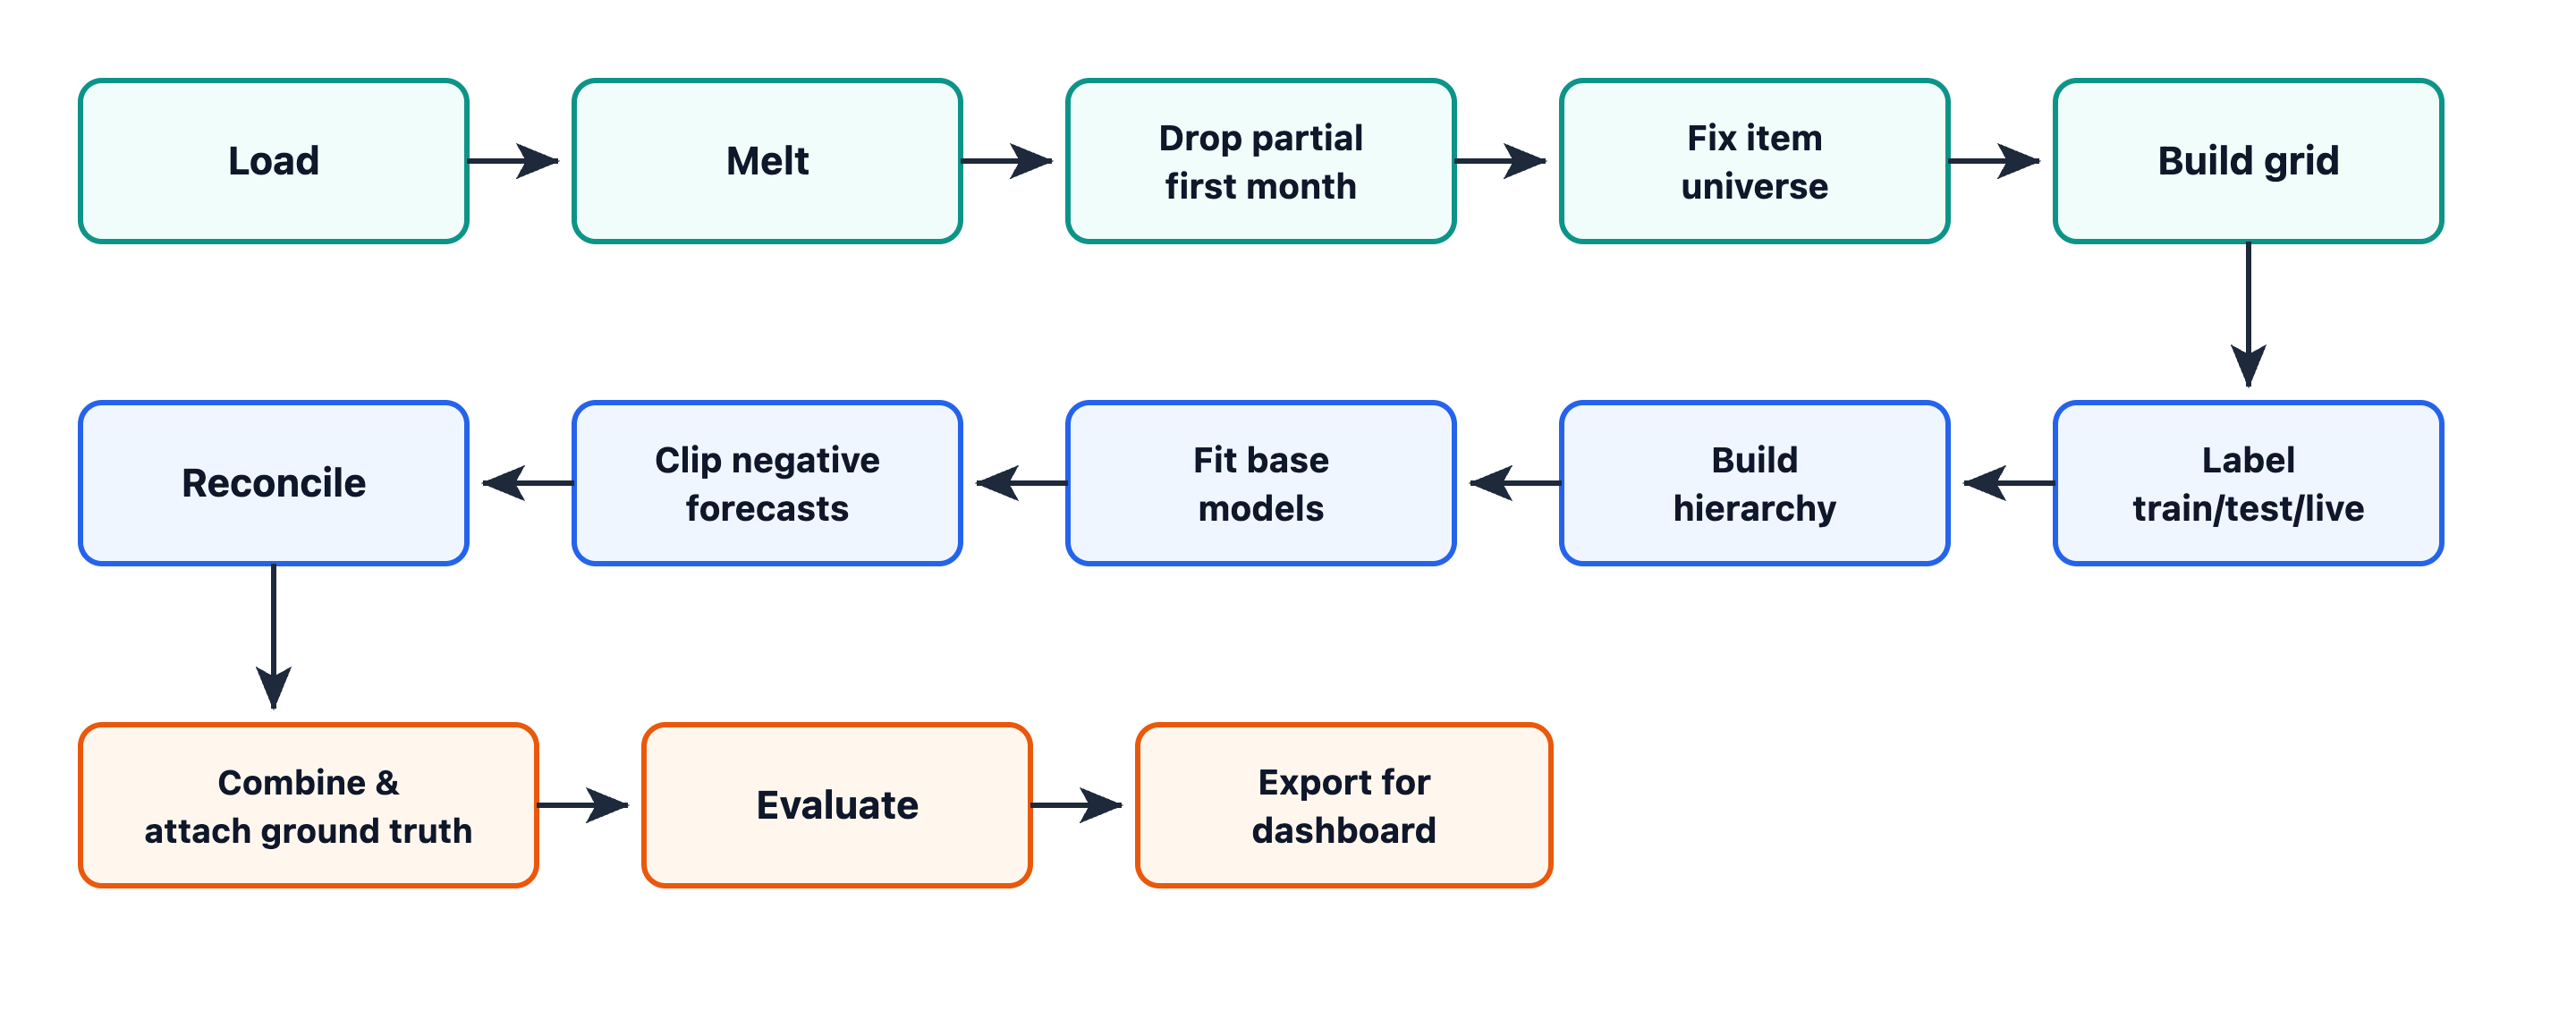
\includegraphics[width=1\linewidth]{Images/06ApplicationDevelopment/pipelineFlowDiagram}
	\caption{The full pipeline, from loading the raw M5 data to exporting the dashboard's Parquet files.}\label{fig:pipelineFlow}
\end{figure}


No static exported plot from the pipeline notebook itself is included alongside this diagram: the notebook's one visualisation step calls an interactive Plotly helper to spot-check a handful of reconciled series, and produces no saved image file to draw on here.

\section{Naming, Parameter, and Error-Handling Conventions}
\label{sec:namingConventions}

Three conventions run through the pipeline code shown above and are worth stating explicitly, since they are what keeps the notebook and the Streamlit dashboard from silently drifting apart as either one changes.

\textbf{Naming.} \texttt{config.py} is the single naming authority for every column and identifier used in this chapter: the hierarchy columns (\texttt{COL\_TOTAL} through \texttt{COL\_ITEM}), the aggregation \texttt{SPEC} passed to \texttt{aggregate()}, the series identifier \texttt{ID\_COL}, and the period label column \texttt{CAT\_LABEL\_COL} are all read from \texttt{cfg} rather than typed out again in the pipeline notebook. Nothing in this chapter hard-codes a column name.

\textbf{Parameter handling.} The three time-window boundaries (the train/test split date, the forecast start date, and the forecast end date) and \texttt{SEASON\_LENGTH} are likewise centralised in \texttt{config.py}, so that the 12-month test horizon and 7-month live horizon computed in Section~\ref{sec:modelFitting} are always derived from the same dates the dashboard uses to shade its train/test/live regions, rather than a second, independently maintained copy of those dates.

\textbf{Error handling.} \texttt{fallback\_model=HistoricAverage()} (Section~\ref{sec:modelFitting}) is the pipeline's only error-handling mechanism for model fitting: rather than raising on a series ETS or Theta cannot fit, the pipeline substitutes the fallback forecast for that series alone and continues. The fallback-rate check in Section~\ref{sec:testingValidation} finds this happens for 699 of the 30,354 series in the hierarchy (2.30\%), identically for both ETS and Theta.

\section{Testing \& Validation}
\label{sec:testingValidation}

Before any of the accuracy figures in Chapter~\ref{chap:evaluation} are treated as meaningful, the pipeline runs three checks against its own output, plus the shape-integrity assertion already shown in Section~\ref{sec:combiningResults}.

\textbf{Coherence check.} Actual sales satisfy $y_t = S b_t$ exactly at every time step (Section~\ref{sec:hierarchicalCoherence}), and HistoricAverage forecasts each series as a plain average of its own past values (Section~\ref{subsec:histAvg}). Averaging both sides of that identity over time shows HistoricAverage's own base forecasts already satisfy the same relationship, $\overline{y} = S\bar{b}$, without any reconciliation step at all: its forecasts are coherent by construction, not by correction. Bottom-Up's reconciliation matrix, $G = [\mathbf{0} \mid I]$ (Section~\ref{subsec:bottomUp}), discards every base forecast above the bottom level and rebuilds the rest through $S$ -- exactly the identity HistoricAverage's forecasts already satisfy -- so applying Bottom-Up to them should barely change anything. Comparing HistoricAverage's base forecast against its Bottom-Up-reconciled counterpart, matched on \texttt{(unique\_id, date)}, gives a maximum absolute difference of 0.146244 -- consistent with the near-zero result this check is designed to confirm, with the small residual attributable to floating-point accumulation across tens of thousands of summed series rather than to a broken merge or reconciliation step.

\textbf{Top-Down root-invariance check.} With a single "Total" root in place, and Top-Down's $G$ matrix constructed so that only the top-level base forecast is ever read and every other base forecast is discarded entirely (Section~\ref{subsec:topDown}), the reconciled Total forecast is definitionally the same number the base model already produced at that node -- Top-Down should never alter the top-level forecast, only redistribute it downward. Comparing ETS's base and Top-Down-reconciled forecasts at the "Total" node gives a maximum absolute difference of 0.000000, confirming the root fix from Section~\ref{sec:totalRoot} holds and that the reconciled root has not drifted from the base forecast it should equal exactly.

\textbf{Fallback-rate check.} Counting, per series rather than per row, how often ETS or Theta produced exactly the HistoricAverage forecast at every horizon gives the 2.30\% figure already stated in Section~\ref{sec:namingConventions}: 699 of 30,354 series for ETS, and the identical 699 of 30,354 for Theta.

Table~\ref{table:validationChecks} summarises all three checks against what each one is designed to confirm.

\begin{table}[htbp]
	\centering
	\small
	\caption{Summary of the pipeline's built-in validation checks.}
	\label{table:validationChecks}
	\begin{tabularx}{\linewidth}{@{} l X r @{}}
		\toprule
		\textbf{Check} & \textbf{Confirms} & \textbf{Result} \\
		\midrule
		Coherence & \textit{HistoricAverage} is coherent by construction; Bottom-Up should barely change it & max diff 0.146244 \\
		\addlinespace
		Top-Down root-invariance & The Total forecast is never altered by Top-Down, only redistributed & max diff 0.000000 \\
		\addlinespace
		Fallback rate & How often ETS/Theta fall back to \textit{HistoricAverage} & 699 / 30,354 (2.30\%) \\
		\bottomrule
	\end{tabularx}
\end{table}

All three checks pass as designed, and the shape-integrity assertion from Section~\ref{sec:combiningResults} raises no error, so the 576,726-row combined forecast table carried into Chapter~\ref{chap:evaluation} is taken to be trustworthy. The business implications of this test protocol and of the 2.30\% fallback rate are discussed alongside the accuracy results in Chapter~\ref{chap:evaluation}.